\documentclass{style/ucasproposal}

\usepackage{style/commons}
\usepackage{style/custom}
\usepackage{pdfpages}
\usepackage[cache=false,outputdir=tmp]{minted}

\setmonofont{Fira Code}
\usemintedstyle{trac}
\newcommand{\cinline}[1]{\mintinline[style=trac]{c}{#1}}

\setcounter{tocdepth}{2}

\begin{document}

\pagenumbering{roman}

\includepdf[page={1}]{pages/fake-cover.pdf}

\tableofcontents

\clearpage
\pagenumbering{arabic}

\section{界面说明}
% ---------------------------------
\subsection{开始界面}

打开游戏,则进入开始界面。上方是标题栏,正中央是开始菜单,一共有4个按钮:
\begin{itemize}
    \item \textbf{New Game}:新的游戏
    \item \textbf{Load Game}:加载存档
    \item \textbf{Ranking}:排行榜/最高分
    \item \textbf{Help}:帮助界面
\end{itemize}

\begin{center}
\begin{figure}[H]
\center
    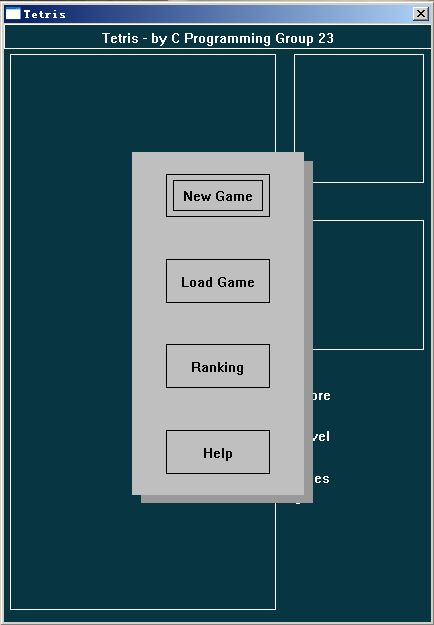
\includegraphics[width=0.7\textwidth]{./img/manual/1-start.png}
\end{figure}
开始界面
\end{center}

% ---------------------------------
\subsection{新的游戏}

在主界面点击"New Game",则进入游戏界面,开始一局新的游戏。
\begin{center}
\begin{figure}[H]
\center
    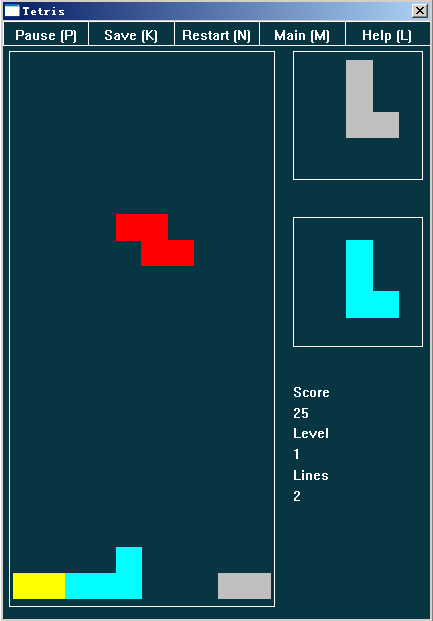
\includegraphics[width=0.7\textwidth]{./img/manual/2-play.png}
\end{figure}
游戏界面
\end{center}

中央大框内是游戏区域,方块从顶部生成,然后按一定速度落下。

右侧从上到下第一个框显示\textbf{下一个方块},其下方的框显示玩家\textbf{暂存的方块}。
有关方块暂存的信息,请点击跳转到\hyperref[hold]{“方块暂存”}一节。

右下角从上到下分别显示\textbf{当前分数}、\textbf{当前难度等级}、\textbf{已消除行数}。

点击可跳转到相应小节:\hyperref[score]{“分数计算与难度等级”}。

上方是游戏菜单,分别对应:
\begin{itemize}
    \item \textbf{Pause (P)}:暂停游戏
    \item \textbf{Save (K)}:保存当前游戏进度
    \item \textbf{Restart (N)}:重新开始
    \item \textbf{Main (M)}:回到开始界面
    \item \textbf{Help (L)}:帮助界面
\end{itemize}

括号中的字母代表\textbf{快捷键},按下键盘上对应字母即可触发相应的事件。

% ---------------------------------
\subsection{暂停界面}
在游戏过程中,点击\textbf{Pause (P)},或按下\textbf{快捷键 P},会暂停游戏,并在屏幕中央显示一个对话框,
提示游戏暂停。同时\textbf{Pause (P)}按钮文字变为\textbf{Resume (P)}。
\begin{center}
\begin{figure}[H]
\center
    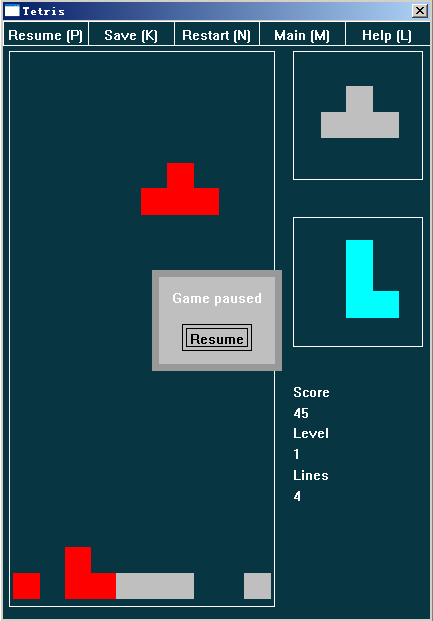
\includegraphics[width=0.7\textwidth]{./img/manual/3-pause.png}
\end{figure}
暂停界面
\end{center}

要继续游戏,可以按下对话框的"Resume"按钮,或选择菜单中的\textbf{Resume (P)},
或按下\textbf{快捷键 P}。同时,菜单栏的其余4个按钮仍然可以点击并触发相应事件。

% ---------------------------------
\subsection{存档加载}
在主界面点击"Load Game",则进入存档加载模式。

在屏幕中央会显示一个对话框,提示输入用户名,以加载对应的存档。
\begin{center}
\begin{figure}[H]
\center
    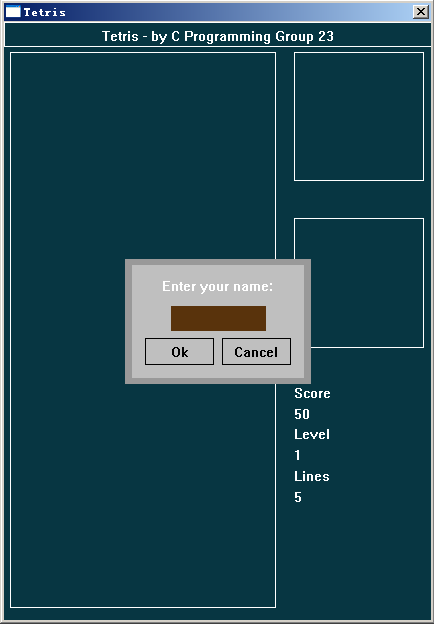
\includegraphics[width=0.7\textwidth]{./img/manual/10-load.png}
\end{figure}
输入用户名以加载
\end{center}

如果找到对应的存档,则加载,并绘制相应的方块与数据,提示用户操作成功:
\begin{center}
\begin{figure}[H]
\center
    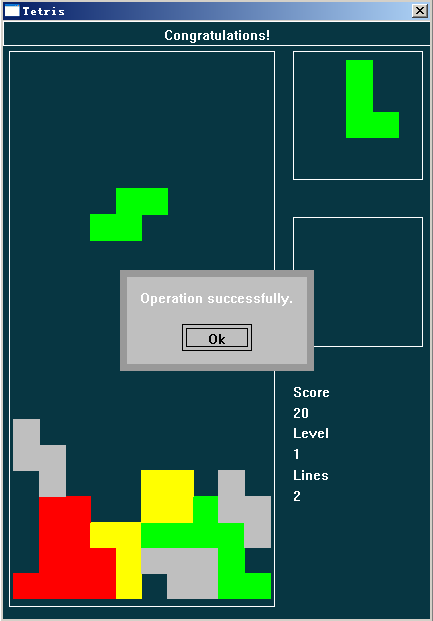
\includegraphics[width=0.7\textwidth]{./img/manual/5-save-or-load-success.png}
\end{figure}
存档加载成功
\end{center}

如果未找到对应的存档,或\textbf{存档格式不正确导致读取失败},则提示用户读取失败:
\begin{center}
\begin{figure}[H]
\center
    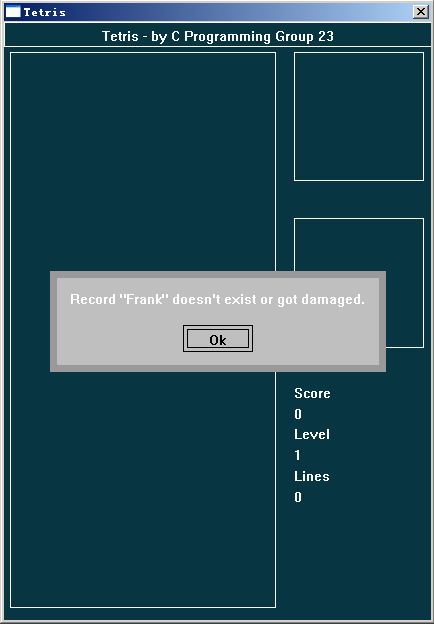
\includegraphics[width=0.7\textwidth]{./img/manual/11-load-fail.png}
\end{figure}
存档加载失败
\end{center}

% ---------------------------------
\subsection{进度保存}
在游戏过程中,点击\textbf{Save (K)},或按下\textbf{快捷键 K},会暂停游戏,
并在屏幕中央显示一个对话框,提示输入用户名。

\begin{center}
\begin{figure}[H]
\center
    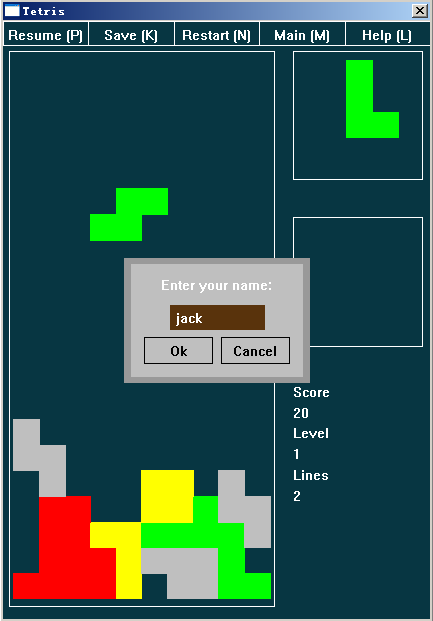
\includegraphics[width=0.7\textwidth]{./img/manual/4-save.png}
\end{figure}
存档保存界面
\end{center}

输入后按下"Ok",则会保存当前游戏进度;点击"Cancel",则继续游戏。
同时,菜单栏的其余4个按钮仍然可以点击并触发相应事件。

保存结果无论成功还是失败,都会用对话框告知用户,例如,保存成功时:

\begin{center}
\begin{figure}[H]
\center
    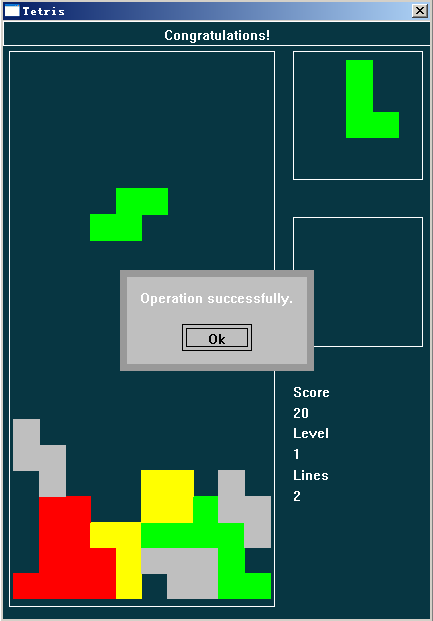
\includegraphics[width=0.7\textwidth]{./img/manual/5-save-or-load-success.png}
\end{figure}
存档保存成功
\end{center}

% ---------------------------------
\subsection{重新开始/回主菜单}
在游戏过程中,点击\textbf{Restart (N)},或按下\textbf{快捷键 N},会暂停游戏,
并在屏幕中央显示一个对话框,让用户确认是否舍弃当前进度,重新开始游戏。

\begin{center}
\begin{figure}[H]
\center
    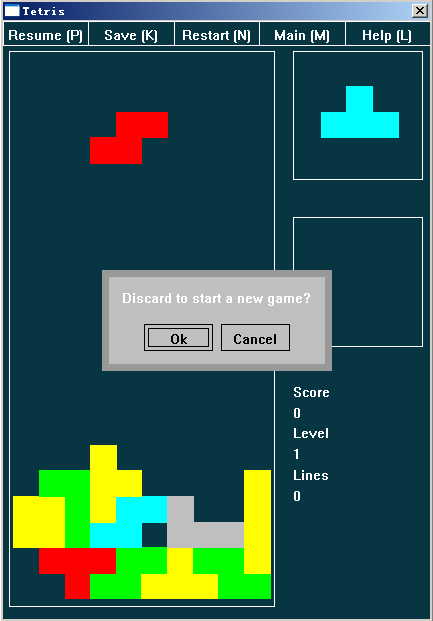
\includegraphics[width=0.7\textwidth]{./img/manual/6-restart.png}
\end{figure}
是否重新开始
\end{center}

按下"Ok",则会重新开始游戏;点击"Cancel",则继续游戏。
同时,菜单栏的其余4个按钮仍然可以点击并触发相应事件。

回到主菜单按钮\textbf{Main (M)}同理。

% ---------------------------------
\subsection{分数记录保存}
游戏结束时,会用对话框提示用户得分,并询问是否保存:
\begin{center}
\begin{figure}[H]
\center
    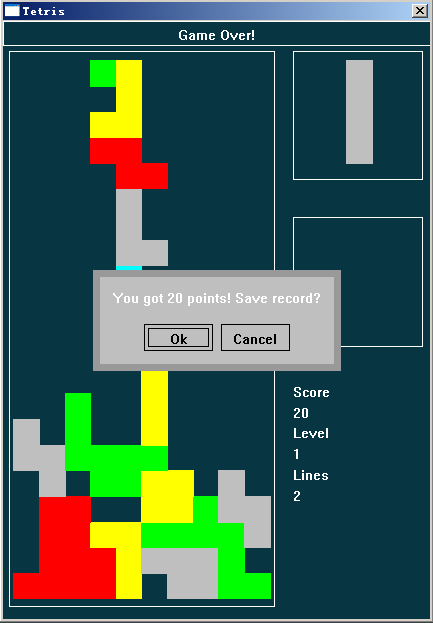
\includegraphics[width=0.7\textwidth]{./img/manual/13-record-save.png}
\end{figure}
分数提示
\end{center}

如点击"Cancel",则返回主菜单;点击"Ok",则会询问玩家姓名并保存分数记录,
保存结果成功与否会用对话框提示用户,流程与保存存档时基本一致,不再赘述。

% ---------------------------------
\subsection{帮助界面}
在游戏中或主菜单点击"Help",则进入帮助界面。

上方是开发者的说明,点击"GitHub"按钮可在浏览器打开游戏源码地址。

下方按钮为游戏中用到的控制键,鼠标点击对应的按钮则可显示帮助信息。
\begin{center}
\begin{figure}[H]
\center
    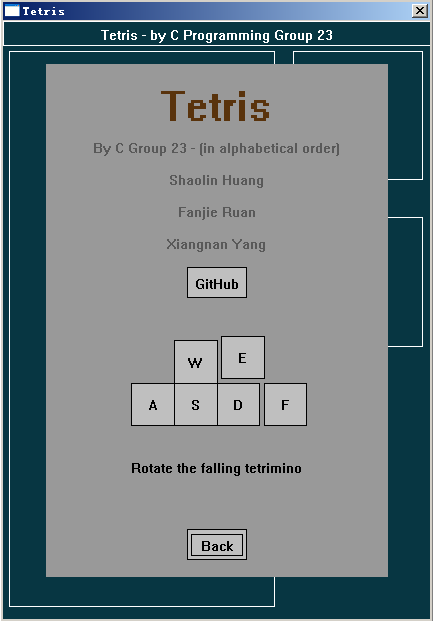
\includegraphics[width=0.7\textwidth]{./img/manual/8-help.png}
\end{figure}
帮助界面
\end{center}


% ---------------------------------
\subsection{排行榜}
在主菜单点击"Ranking",则进入排行榜界面。

排行榜显示前十位玩家的名次、姓名与分数,其中前三位高亮显示。

\begin{center}
\begin{figure}[H]
\center
    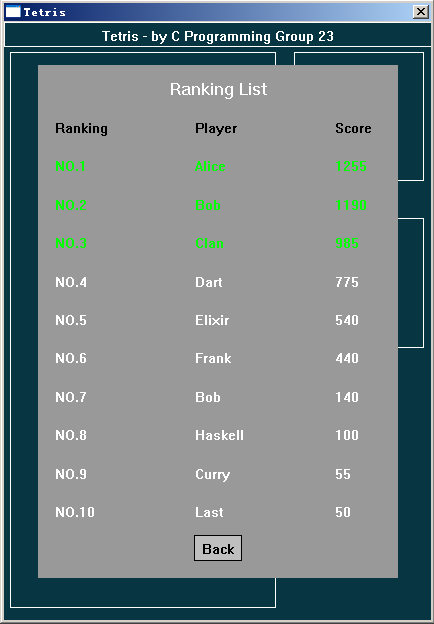
\includegraphics[width=0.7\textwidth]{./img/manual/9-ranking.png}
\end{figure}
排行榜界面
\end{center}


% ---------------------------------
\section{游戏功能说明}
\subsection{分数计算与难度等级}
\label{score}
分数计算采取“阶梯式”计分,即每消除一行,可得到10分的\textbf{基准分},
与此同时,如果同时消除了多行,则每多一行,可得到5分的\textbf{额外分数}。

难度等级最高为5级,刚开始游戏时为一级,每消除10行,则难度增加一级。
难度上升后,方块下落速度会变快。


\subsection{方块暂存}
\label{hold}
\textbf{方块暂存(\textit{Hold})},即玩家可以将当前下落方块暂时保存起来,流程切换到下一个方块;
在需要时,玩家可以将暂存的方块\textbf{释放(\textit{release})}出来代替当前方块,当前方块则被延迟一轮。

在游戏中,按"E"键即可进行暂存/释放,\textbf{释放后一轮之内不能使用该功能}。

方块暂存功能可以丰富游戏内容,调节游戏平衡度,为完全随机的俄罗斯方块游戏\textbf{引入一点确定性}。


\subsection{存档与分数记录}
存档与分数记录保存在 \cinline{saves/} 目录下。

其中,一个存档的文件名为 “用户名” + \cinline{.save}。

分数记录文件名为 \cinline{records} ,以文本方式储存。

(注:如果结束游戏时用户保存的分数没有进入前十名,则在排行榜上不会显示,
但仍然会被储存到该文件中)

\section*{其他说明}

本文档使用 \LaTeX{} 编写,TeX源码(已隐去个人信息): \url{https://github.com/sakamitz/tetris/tree/master/report}.

\end{document}
